\newpage
\section{Previsione del volume di business} \label{ref:previsione}
La previsione del volume di business si basa essenzialmente sulla crescente domanda di cura dovuta all’invecchiamento demografico. Risulterà quindi cruciale indirizzare al meglio le risorse a disposizione, in modo da far fronte alle esigenze dell'istituto.\\
Possiamo vedere nel grafico sottostante l'andamento dell'indice di vecchiaia della città di Milano, dove opera l'istituto Gaetano Pini, in cui è chiara una forte crescita dell'indice di vecchiaia dal 2010 ad oggi, che porta a presupporre una continua crescita anche per l'anno successivo.
\begin{figure}[h!]
	\centering
	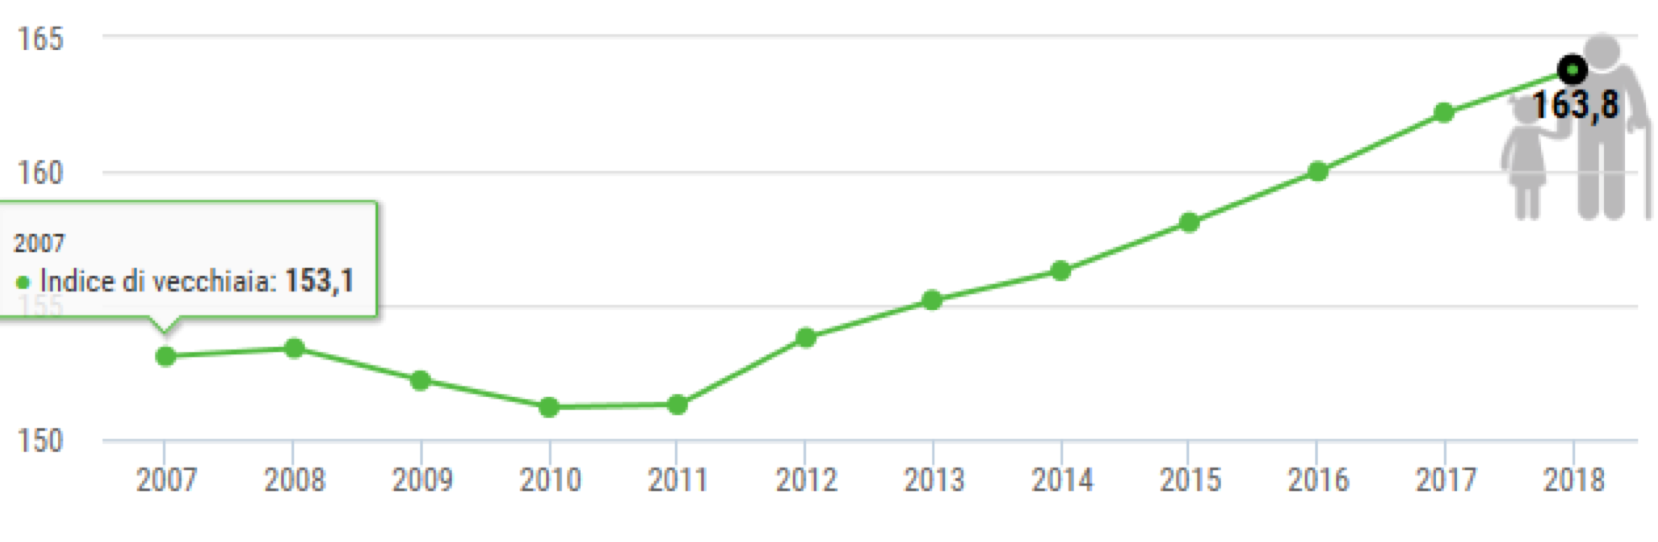
\includegraphics[width=\linewidth]{./img/vecchiaia.jpg}
	\caption{Indice di vecchiaia Milano 2007-2018}\label{fig:vecchiaia}
\end{figure}

Inoltre per il seguente anno l'istituto ha deciso di effettuare diverse variazioni nell'organico e nella gestione che comporteranno una variazione del volume di business. \\
In particolare i cambiamenti previsti per il prossimo anno che incideranno sulle analisi di previsione dei servizi IT sono:
\begin{itemize}
	\item Integrazione del costo della formazione, che porterà ad un aumento di personale in formazione che utilizzerà gli applicativi;
	\item Integrazione dei costi sulla sicurezza, che porterà al miglioramento dell'infrastruttura tecnologica;
	\item Revisione dei costi del personale, che porterà ad un aumento del personale che utilizzerà gli applicativi ed aumento del numero di postazioni IT di lavoro.
\end{itemize}

Tutti e tre i punti elencati sopra porteranno ad un aumento del numero di utilizzatori dei servizi digitali, il che a sua volta porterà ad un ulteriore incremento della base di utenti.